\chapter{Js foundation}

\section{JavaScript Engine}

    JavaScript (\acrshort{js}) engine is a translator between \textit{\acrshort{js} language} and \textit{computer native language} - 0,1  \cite{JavaScriptEngineImage2020}.
    There are tons of \acrshort{js} engines \cite{ECMAScriptEngines}. One of the most famous is google V8 engine. 
    The creator of first \acrshort{js} engine is Brendan Eich cofounder of the Mozilla project, the Mozilla Foundation, and the Mozilla Corporation \cite{BrendanEich}.


    
    \begin{figure}[h]
        \begin{center}
            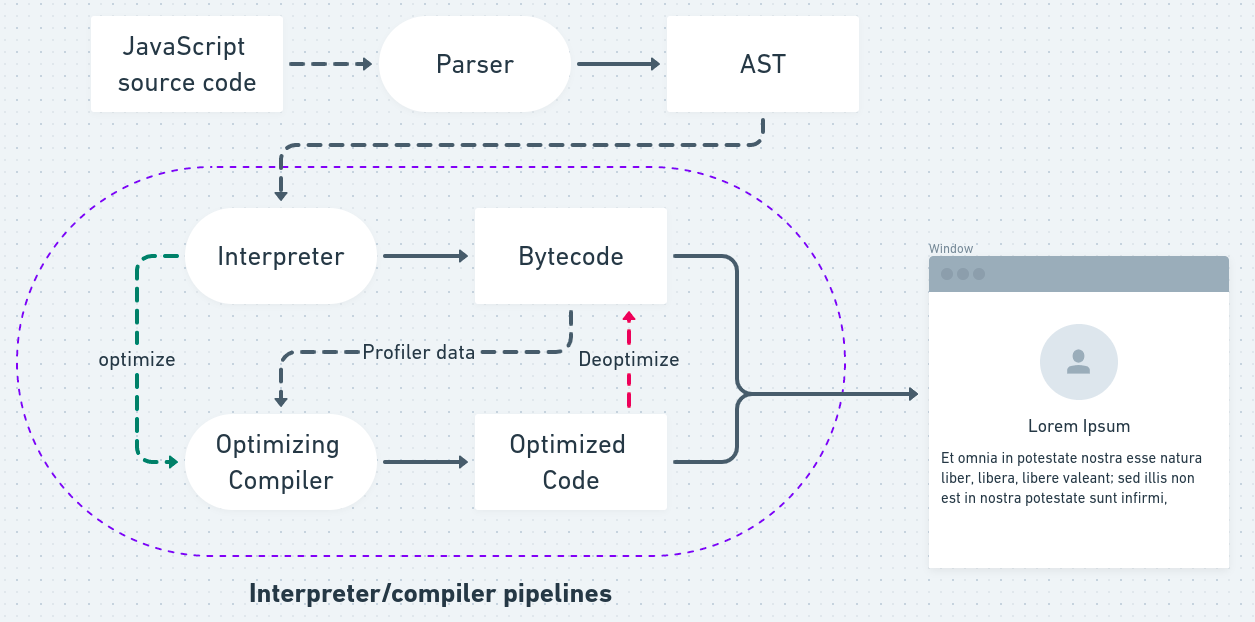
\includegraphics[width=10cm]{01/images/01-js-engine.png}
            \caption[JavaScript engine]{JavaScript engine description  \cite{JavaScriptEngineImage2020}.}
        \end{center}
    \end{figure}

   
